\documentclass[11pt,english]{article}

%%%%%%%%%%%%%%%%%%%%%%%%%%%%%%%%%%%%%%%%%%%%%%%%%%%%%%%%%%%
% Packages
%%%%%%%%%%%%%%%%%%%%%%%%%%%%%%%%%%%%%%%%%%%%%%%%%%%%%%%%%%%

% paper size & margins
\usepackage{fullpage}
\usepackage[showframe=false,margin=1in]{geometry}
\parindent=0pt

% font management
\usepackage{relsize}
\usepackage[T1]{fontenc} % for properly hyphenating words with accented chars
\usepackage[latin1]{inputenc}
\usepackage{babel}

% math
\usepackage{amsmath, amsthm, amssymb}
\usepackage{textcomp}
\usepackage{stmaryrd}
\usepackage{upgreek}
\usepackage{bm}
\usepackage[linesnumbered,ruled,vlined]{algorithm2e}


% assorted
\usepackage{url}
\usepackage{breakurl}
\usepackage{xspace}
\usepackage{comment}
\usepackage{color}
\usepackage{afterpage}
\usepackage{tikz}

%%%%%%%%%%%%%%%%%%%%%%%%%%%%%%%%%%%%%%%%%%%%%%%%%%%%%%%%%%%
% Shortcuts
%%%%%%%%%%%%%%%%%%%%%%%%%%%%%%%%%%%%%%%%%%%%%%%%%%%%%%%%%%%
\newcommand{\hide}[1]{}
\DeclareMathOperator*{\argmin}{arg\,min}
\newtheorem{theorem}{Theorem}[section]
\newtheorem{corollary}{Corollary}[theorem]
\newtheorem{lemma}[theorem]{Lemma}

%%%%%%%%%%%%%%%%%%%%%%%%%%%%%%%%%%%%%%%%%%%%%%%%%%%%%%%%%%%
% Title / Author
%%%%%%%%%%%%%%%%%%%%%%%%%%%%%%%%%%%%%%%%%%%%%%%%%%%%%%%%%%%
\begin{document}

\title{CS7643: Deep Learning \\
Fall 2019\\ HW3 Solutions}
\author{James Hahn}
\maketitle

\setcounter{MaxMatrixCols}{25}
\setlength\arraycolsep{1pt}

%%%%%%%%%%%%%%%%%%%%%%%%%%%%%%%%%%%%%%%%%%%%%%%%%%%%%%%%%%%
% Body
%%%%%%%%%%%%%%%%%%%%%%%%%%%%%%%%%%%%%%%%%%%%%%%%%%%%%%%%%%%

\section{Recurrent Neural Network}

\begin{enumerate}
	\item The answer can be found below: \\\\
	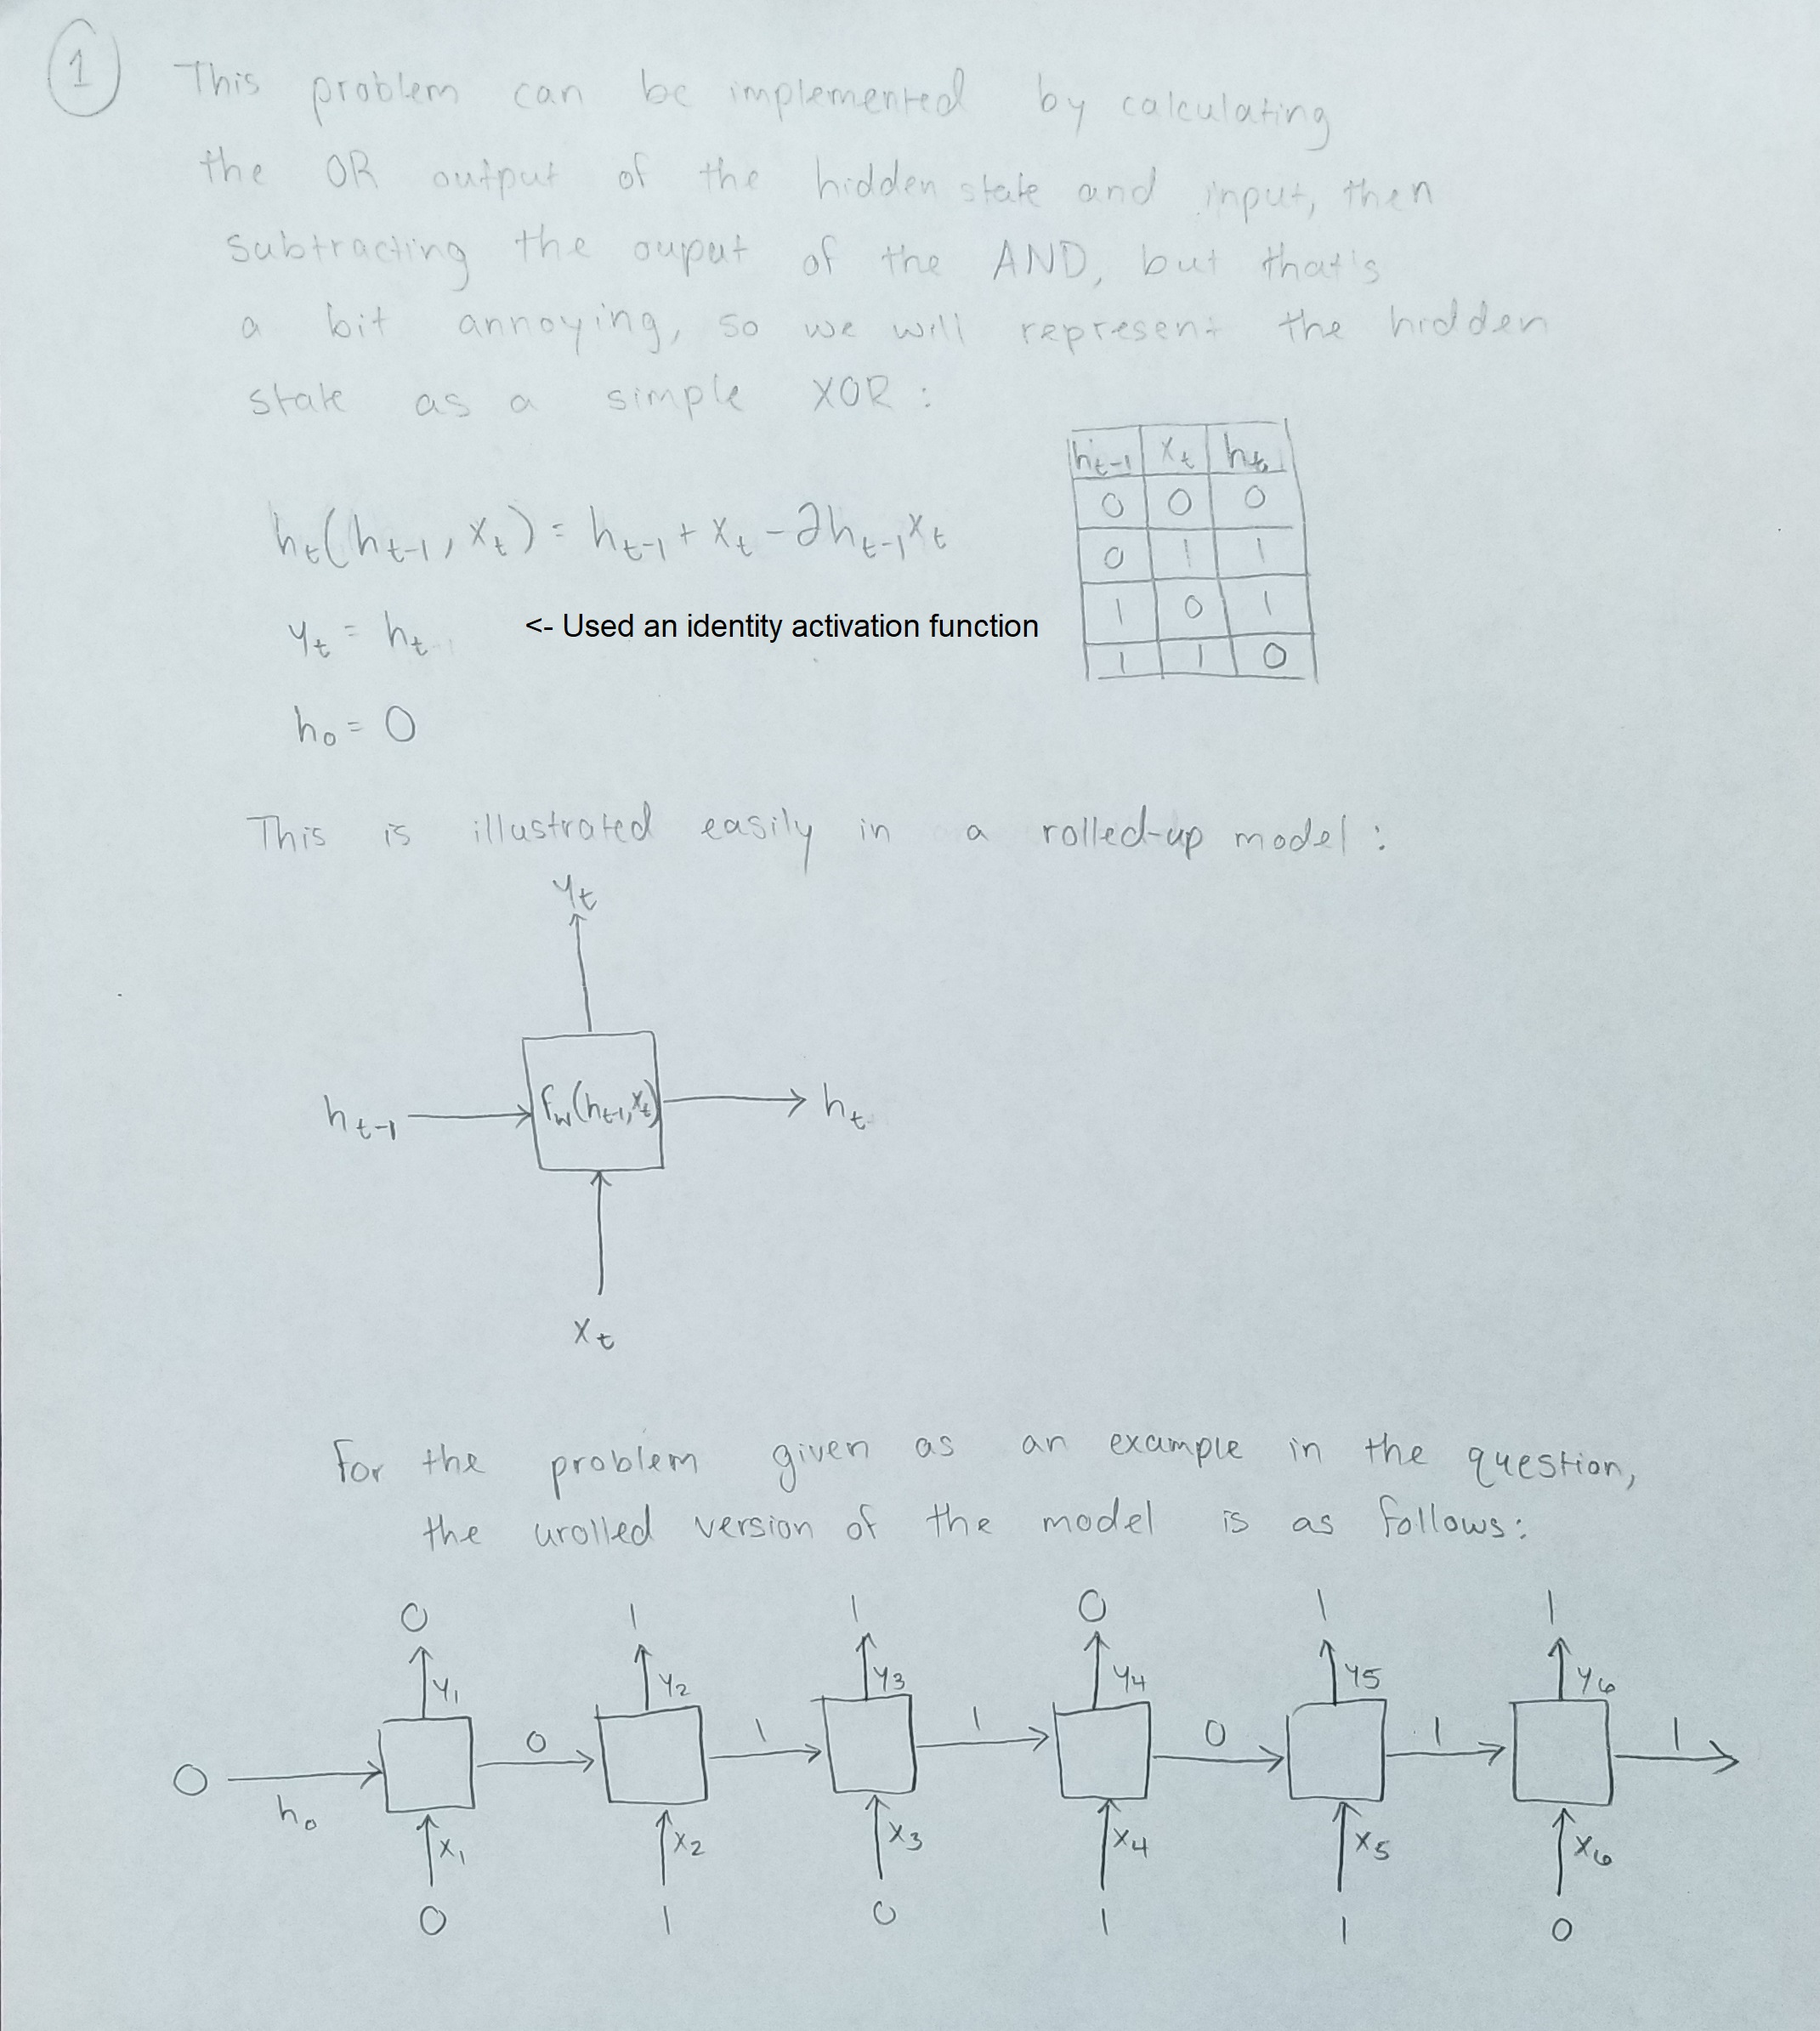
\includegraphics[scale=0.15]{1-1.jpg} \pagebreak
	\item The answer can be found below: \\\\
	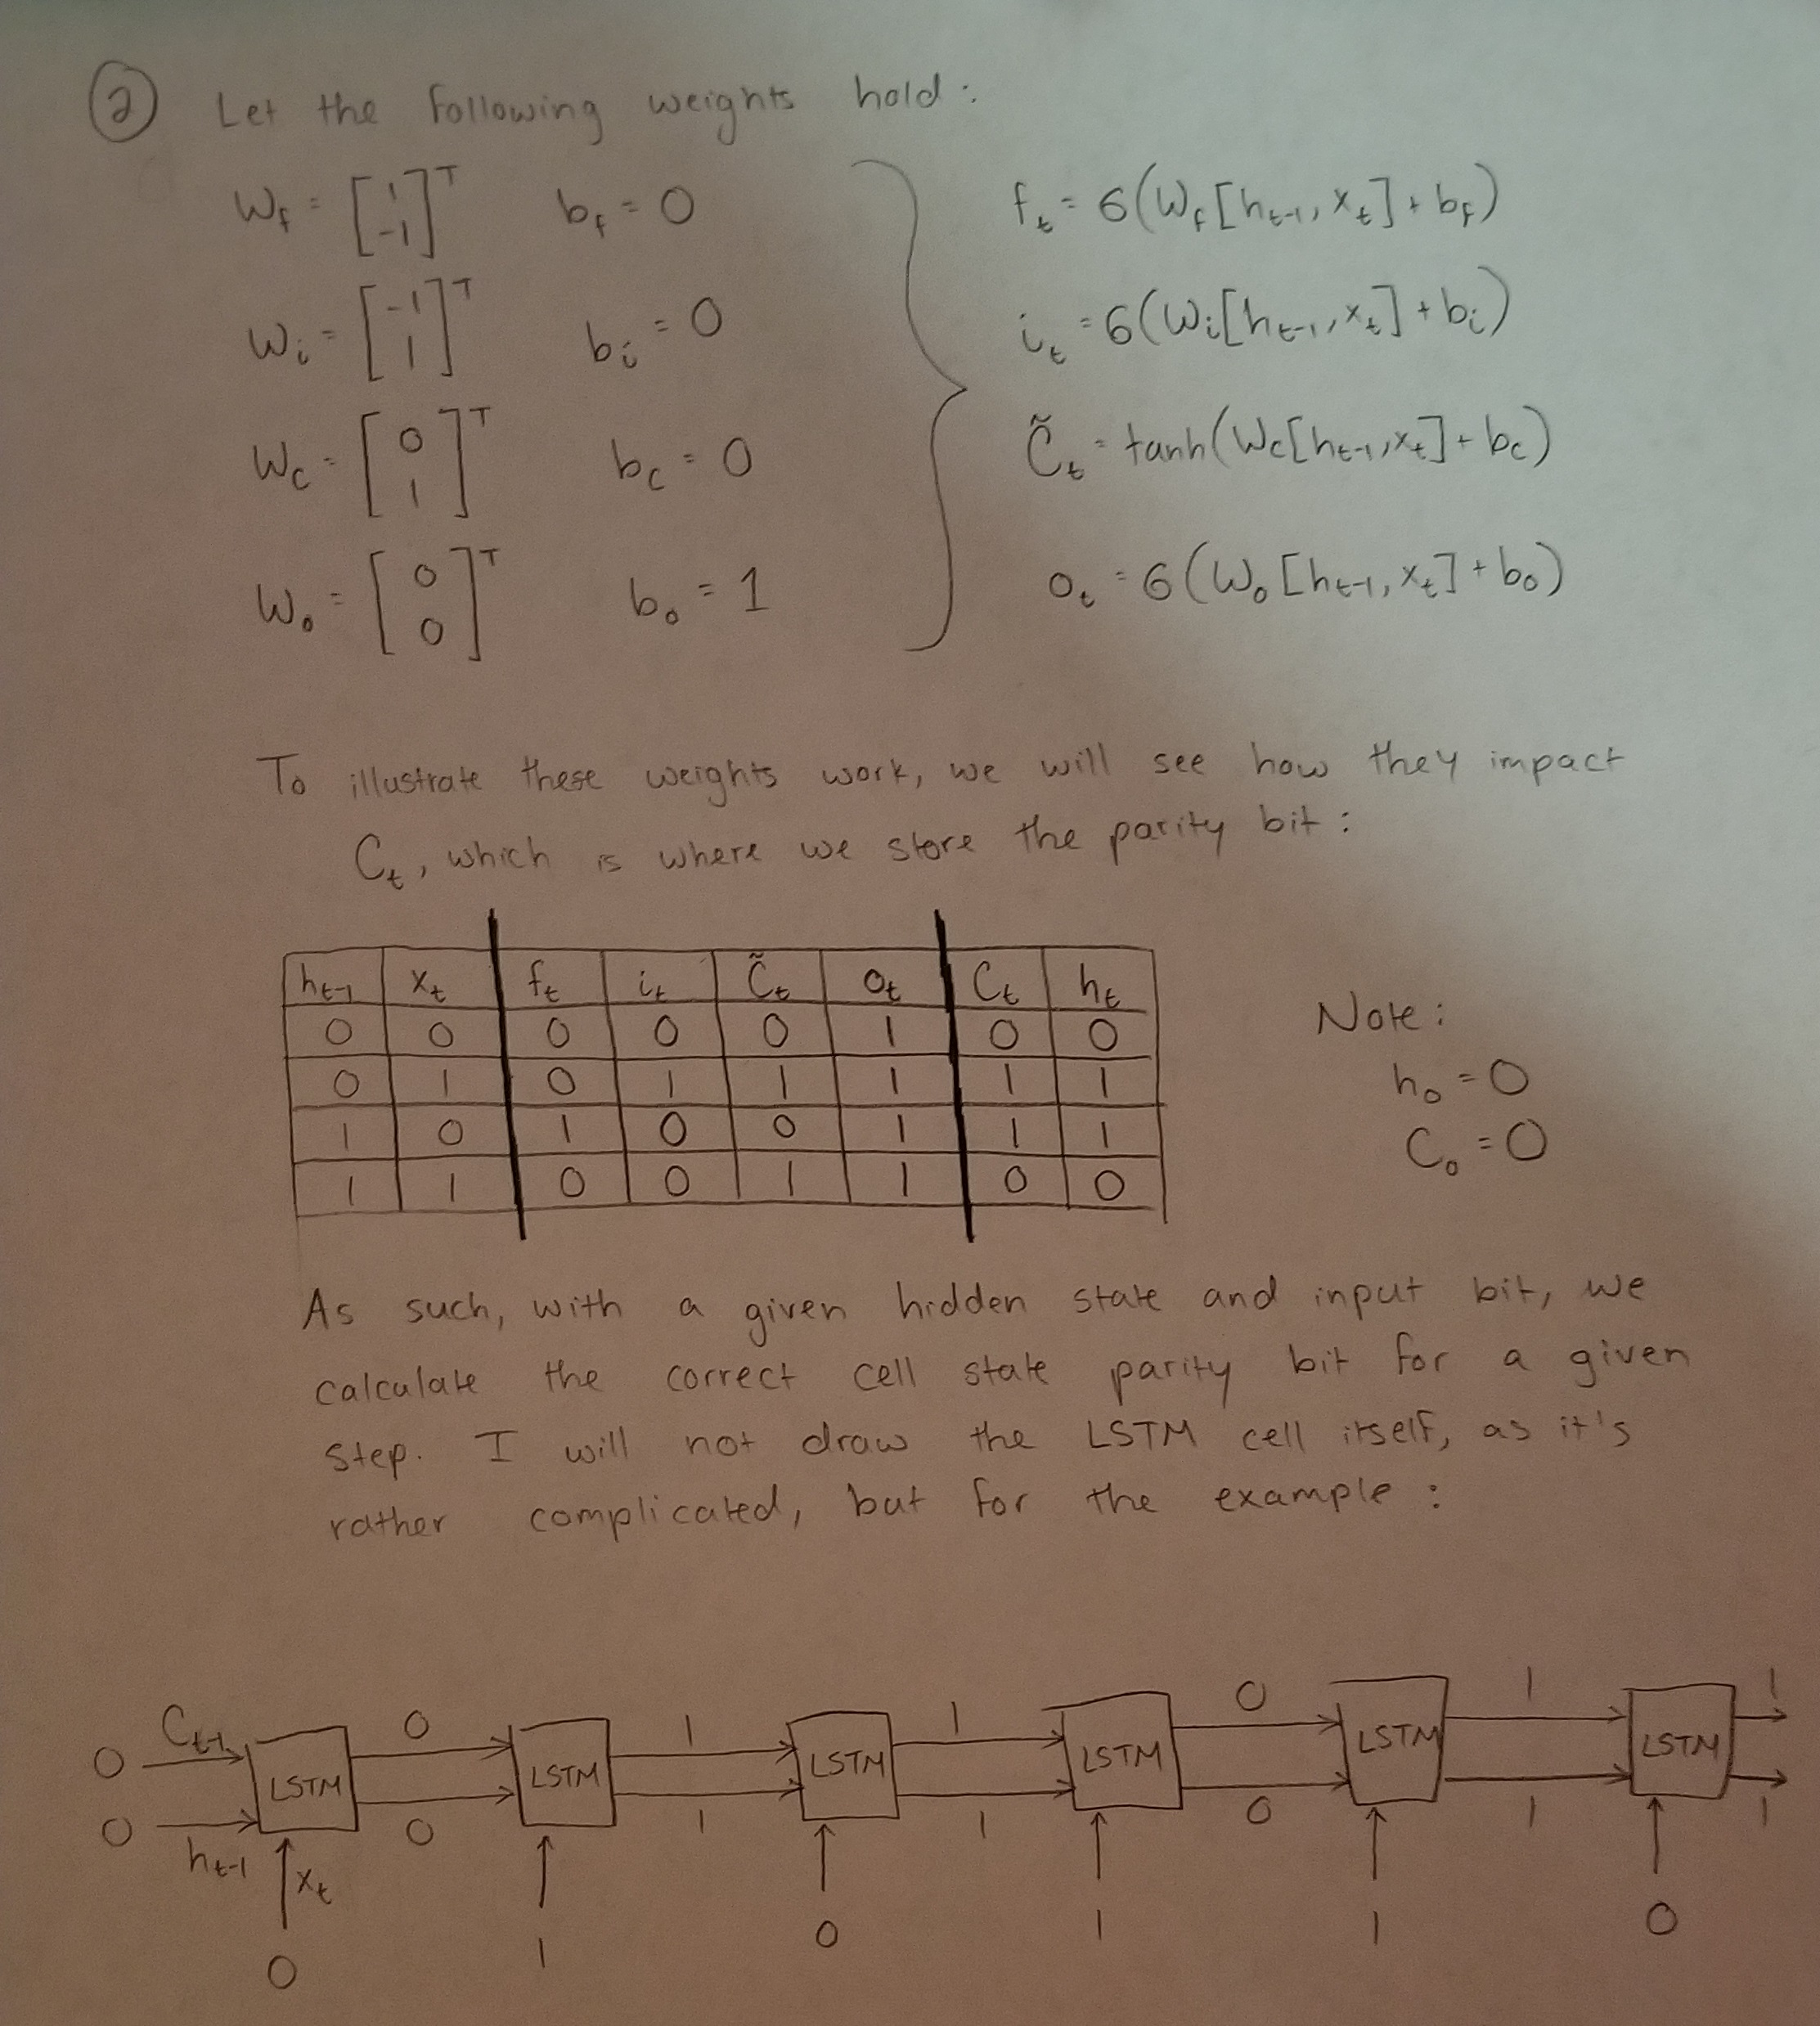
\includegraphics[scale=0.15]{1-2.jpg} \pagebreak
	\item We want to show at a given step $i$ of the beam search, if $\textit{best}_{\leq i}$ exists, then all other beam scores $B_i$ at iteration $i$ will be worse than $\textit{best}_{\leq i}$, so it is not worth exploring the search.
	
	First, we know for a given $B_i$ list of length $i$, its probably $p(y_i | x, y_{<i}) = s$. Second, we know $\sum_x p(y_{i+1} | x, y_{<i+1}) = 1$. As such, for a given $x$, $p(y_{i+1} | x, y_{<i+1}) = p(x)p(y_{i+1} | y_{<i+1})$. This means if $p(x) \in [0, 1]$, then the current score $s$ at $B_i$ will have the value $s_{i+1} = p(x)\cdot s \leq s$ for the list $B_{i+1}$. As such, if $B_i$ has probability $s$ that's lower than $\textit{best}_{\leq i}$, then $B_{i+1}$ will have score $s_{i+1}$ that is at best as high as $s$, so it is useless exploring that set of prefixes. To conclude, $\textit{best}_{\leq i}$ will still be the optimal solution for all iterations $i$ and beyond.
	
	$\therefore$ $\textit{best}_{\leq i}$ is the overall highest-probability completed hypothesis and future steps will be no better than it \pagebreak 
	\item We want to show in a vanilla RNN, with a basic recurrence relation (i.e. $h_t = W^T h_{t-1}$), there exists both the vanishing and exploding gradient problem.
	
	First, we notice $h_t = W^T h_{t-1} = (W^T)^2 h_{t-2} = \cdots = (W^T)^t h_0$.
	
	So, $\frac{dh_t}{dh_0} = (W^T)^t$. Let $W$ be size $n\times n$. We know $W$ can be decomposed into its eigenvalues and eigenvectors such that $W = Q\Lambda Q^{-1}$, where $Q$ is a square $n\times n$ matrix holding the eigenvectors in its columns and $\Lambda$ is a diagonal matrix where each element along the diagonal corresponds to its respective eigenvector in $Q$.
	
	Now, we get $\frac{dh_t}{dh_0} = (W^T)^t \\
	= ([Q\Lambda Q^{-1}]^T)^t \\
	= ([Q^{-1}]^T\Lambda^T Q^T)^t \qquad(\text{NOTE: } (ABC)^T = C^TB^TA^T)\\
	= ([Q^{-1}]^T\Lambda Q^T)^t \qquad(\text{NOTE: } \text{If } A \text{ is diagonal, then } A = A^T) \\
	= [Q^{-1}]^T\Lambda^t Q^T$\\
	
	So, we see the gradient we are trying to calculate heavily relies on the eigenvalues in $\Lambda$. We are given that $\rho(W) = max\{|\lambda_1|, \cdots, |\lambda_n|\}$. Assume $t$ itself is relatively large (i.e. we are doing deep learning, otherwise the whole vanishing/exploding gradients thing isn't a concern in the first place). If $\rho(W)$ is greater than 1, then at least one value of $\Lambda^t$ will exponentially grow toward $\pm\infty$, and the gradient itself will eventually be multiplied by this $\pm\infty$ value, hence the term ``exploding gradients''. On the other hand, if $\rho(W)$ is less than 1, then all eigenvalues will be somewhat close to 0, and the elements of $\Lambda^t$ will converge to 0 (due to repeated multiplications), leading to the gradient becoming almost completely 0, hence the term ``vanishing gradient''.
	
	$\therefore$ We have shown in a vanilla RNN, with a simple recurrence relation, the vanishing/exploding gradient problem exists purely due to the eigenvalues of $W$ $\qed$
\end{enumerate}

\end{document}
